

\tikzset{every picture/.style={line width=0.75pt}} %set default line width to 0.75pt        

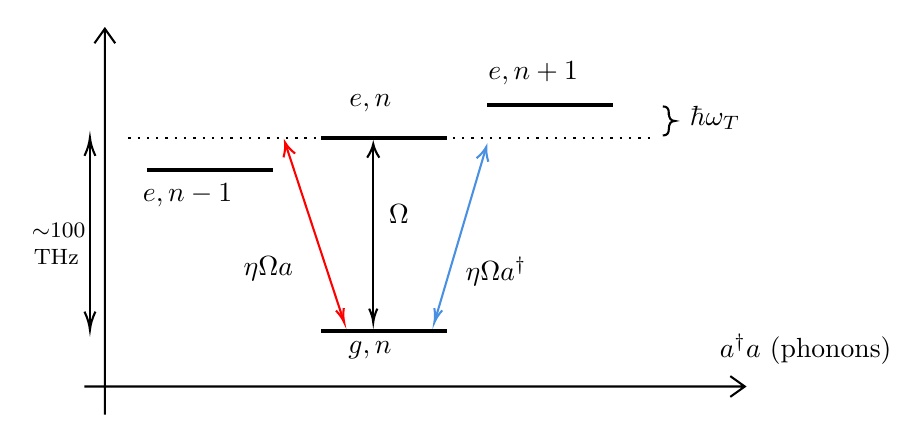
\begin{tikzpicture}[x=0.75pt,y=0.75pt,yscale=-1,xscale=1]
%uncomment if require: \path (0,199); %set diagram left start at 0, and has height of 199

%Shape: Axis 2D [id:dp6304689266356812] 
\draw  (37.83,176.32) -- (356.01,176.32)(47.68,3.94) -- (47.68,189.88) (349.01,171.32) -- (356.01,176.32) -- (349.01,181.32) (42.68,10.94) -- (47.68,3.94) -- (52.68,10.94)  ;
%Straight Lines [id:da9096429015684652] 
\draw [line width=1.5]    (68,72) -- (128.47,72) ;
%Straight Lines [id:da10599775473097062] 
\draw [line width=1.5]    (152,149.5) -- (212.47,149.5) ;
%Straight Lines [id:da5859149964722625] 
\draw [line width=1.5]    (152,56.5) -- (212.47,56.5) ;
%Straight Lines [id:da32072281915513823] 
\draw [line width=1.5]    (232,40.5) -- (292.47,40.5) ;
%Straight Lines [id:da09610392103973153] 
\draw    (40.5,58.44) -- (40.5,147) ;
\draw [shift={(40.5,149)}, rotate = 270] [color={rgb, 255:red, 0; green, 0; blue, 0 }  ][line width=0.75]    (8.74,-2.63) .. controls (5.56,-1.12) and (2.65,-0.24) .. (0,0) .. controls (2.65,0.24) and (5.56,1.12) .. (8.74,2.63)   ;
\draw [shift={(40.5,56.44)}, rotate = 90] [color={rgb, 255:red, 0; green, 0; blue, 0 }  ][line width=0.75]    (8.74,-2.63) .. controls (5.56,-1.12) and (2.65,-0.24) .. (0,0) .. controls (2.65,0.24) and (5.56,1.12) .. (8.74,2.63)   ;
%Straight Lines [id:da3310136117207533] 
\draw [color={rgb, 255:red, 255; green, 0; blue, 0 }  ,draw opacity=1 ]   (135.12,60.67) -- (162.34,143.47) ;
\draw [shift={(162.97,145.38)}, rotate = 251.81] [color={rgb, 255:red, 255; green, 0; blue, 0 }  ,draw opacity=1 ][line width=0.75]    (6.56,-1.97) .. controls (4.17,-0.84) and (1.99,-0.18) .. (0,0) .. controls (1.99,0.18) and (4.17,0.84) .. (6.56,1.97)   ;
\draw [shift={(134.5,58.77)}, rotate = 71.81] [color={rgb, 255:red, 255; green, 0; blue, 0 }  ,draw opacity=1 ][line width=0.75]    (6.56,-2.94) .. controls (4.17,-1.38) and (1.99,-0.4) .. (0,0) .. controls (1.99,0.4) and (4.17,1.38) .. (6.56,2.94)   ;
%Straight Lines [id:da10284525377100584] 
\draw [color={rgb, 255:red, 74; green, 144; blue, 226 }  ,draw opacity=1 ]   (230.9,62.79) -- (207.03,143.46) ;
\draw [shift={(206.47,145.38)}, rotate = 286.48] [color={rgb, 255:red, 74; green, 144; blue, 226 }  ,draw opacity=1 ][line width=0.75]    (6.56,-1.97) .. controls (4.17,-0.84) and (1.99,-0.18) .. (0,0) .. controls (1.99,0.18) and (4.17,0.84) .. (6.56,1.97)   ;
\draw [shift={(231.47,60.88)}, rotate = 106.48] [color={rgb, 255:red, 74; green, 144; blue, 226 }  ,draw opacity=1 ][line width=0.75]    (6.56,-2.94) .. controls (4.17,-1.38) and (1.99,-0.4) .. (0,0) .. controls (1.99,0.4) and (4.17,1.38) .. (6.56,2.94)   ;
%Straight Lines [id:da5949199879144775] 
\draw    (177,61.5) -- (177,143.38) ;
\draw [shift={(177,145.38)}, rotate = 270] [color={rgb, 255:red, 0; green, 0; blue, 0 }  ][line width=0.75]    (6.56,-1.97) .. controls (4.17,-0.84) and (1.99,-0.18) .. (0,0) .. controls (1.99,0.18) and (4.17,0.84) .. (6.56,1.97)   ;
\draw [shift={(177,59.5)}, rotate = 90] [color={rgb, 255:red, 0; green, 0; blue, 0 }  ][line width=0.75]    (6.56,-2.94) .. controls (4.17,-1.38) and (1.99,-0.4) .. (0,0) .. controls (1.99,0.4) and (4.17,1.38) .. (6.56,2.94)   ;
%Straight Lines [id:da5656279166859981] 
\draw  [dash pattern={on 0.84pt off 2.51pt}]  (59,56.5) -- (310.97,56.5) ;
%Shape: Brace [id:dp5779107364872813] 
\draw   (316.5,55.38) .. controls (318.42,55.38) and (319.38,54.42) .. (319.38,52.49) -- (319.38,52.49) .. controls (319.38,49.75) and (320.34,48.38) .. (322.26,48.38) .. controls (320.34,48.38) and (319.38,47.01) .. (319.38,44.26)(319.38,45.49) -- (319.38,44.26) .. controls (319.38,42.34) and (318.42,41.38) .. (316.5,41.38) ;

% Text Node
\draw (64.5,76.9) node [anchor=north west][inner sep=0.75pt]    {$\ket{e,n-1}$};
% Text Node
\draw (163.5,153.4) node [anchor=north west][inner sep=0.75pt]    {$\ket{g,n}$};
% Text Node
\draw (164,34.4) node [anchor=north west][inner sep=0.75pt]    {$\ket{e,n}$};
% Text Node
\draw (231,18.4) node [anchor=north west][inner sep=0.75pt]    {$\ket{e,n+1}$};
% Text Node
\draw (342.5,149.4) node [anchor=north west][inner sep=0.75pt]    {$a^{\dagger } a$ (phonons)};
% Text Node
\draw (11,90.5) node [anchor=north west][inner sep=0.75pt]  [font=\footnotesize] [align=left] {\begin{minipage}[lt]{17.68pt}\setlength\topsep{0pt}
\begin{center}
$\sim$100\\THz
\end{center}

\end{minipage}};
% Text Node
\draw (220,112.4) node [anchor=north west][inner sep=0.75pt]    {$\eta\Omega a^{\dagger }$};
% Text Node
\draw (113,112.4) node [anchor=north west][inner sep=0.75pt]    {$\eta\Omega a$};
% Text Node
\draw (183,87.4) node [anchor=north west][inner sep=0.75pt]    {$\Omega $};
% Text Node
\draw (328,39.9) node [anchor=north west][inner sep=0.75pt]    {$\hbar\omega _{T}$};


\end{tikzpicture}
